
\section{Hardware}
\label{ServerHardware}

\begin{figure}[H]
\begin{center}
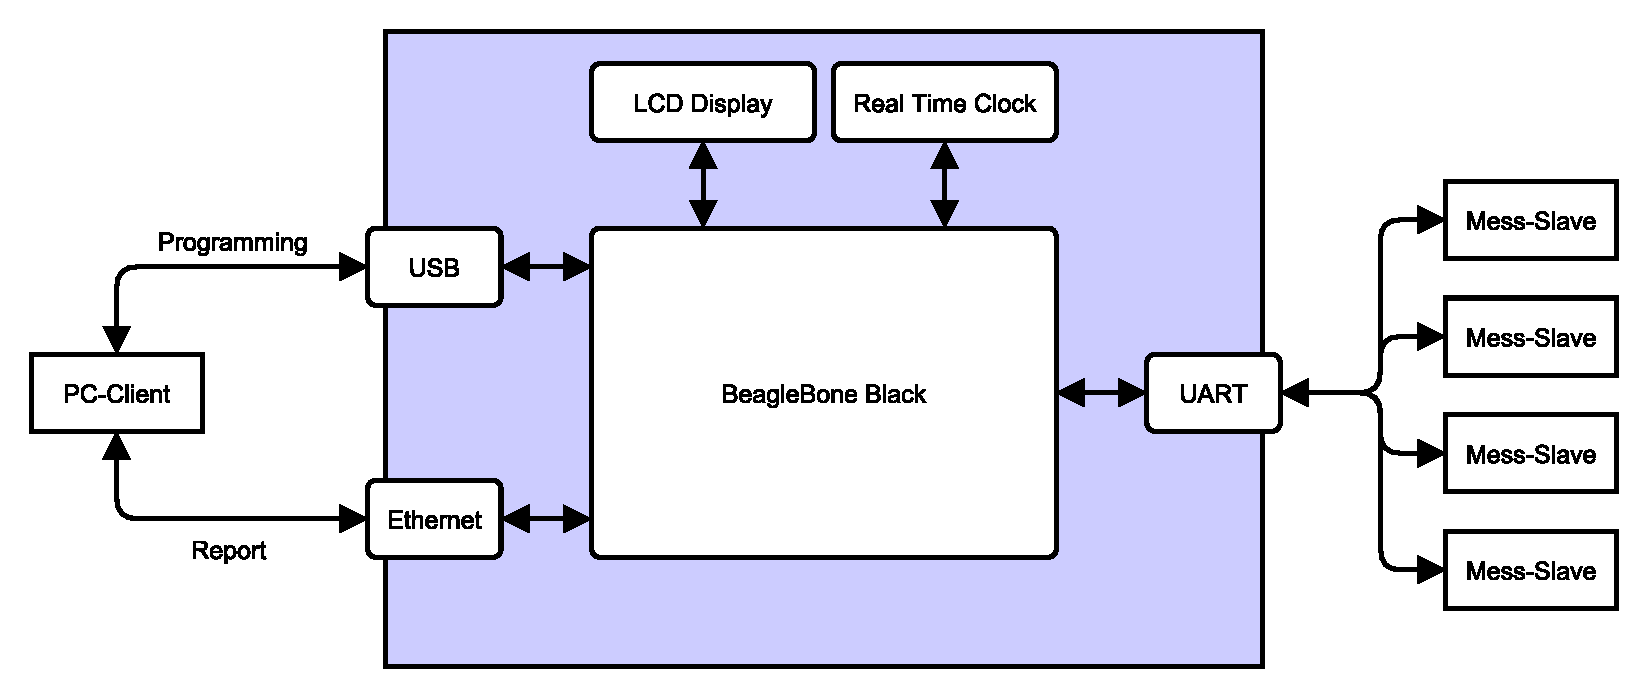
\includegraphics[width=\textwidth ]{img/general/UebersichtMaster.pdf}
\caption{Aufbau Mess-Server}
\label{figure_AufbauBleagleBone}
\end{center}
\end{figure}

Das BeagleBone selbst ist bereits sehr Leistungsstark. Um jedoch weiter Funktionen und Schnittstellen hinzuzufügen, existieren Capes. Ein Cape ist eine für das BeagleBone konzipierte Erweiterung, die direkt auf das BeagleBone aufgesteckt werden kann. Die Treiber vieler dieser Capes sind bereits in dem Betriebssystem des BeagleBones integriert oder werden vom Hersteller bereitgestellt. Somit ist die Inbetriebnahme sehr komfortable.


\begin{figure}[!htb]
\minipage{0.32\textwidth}
  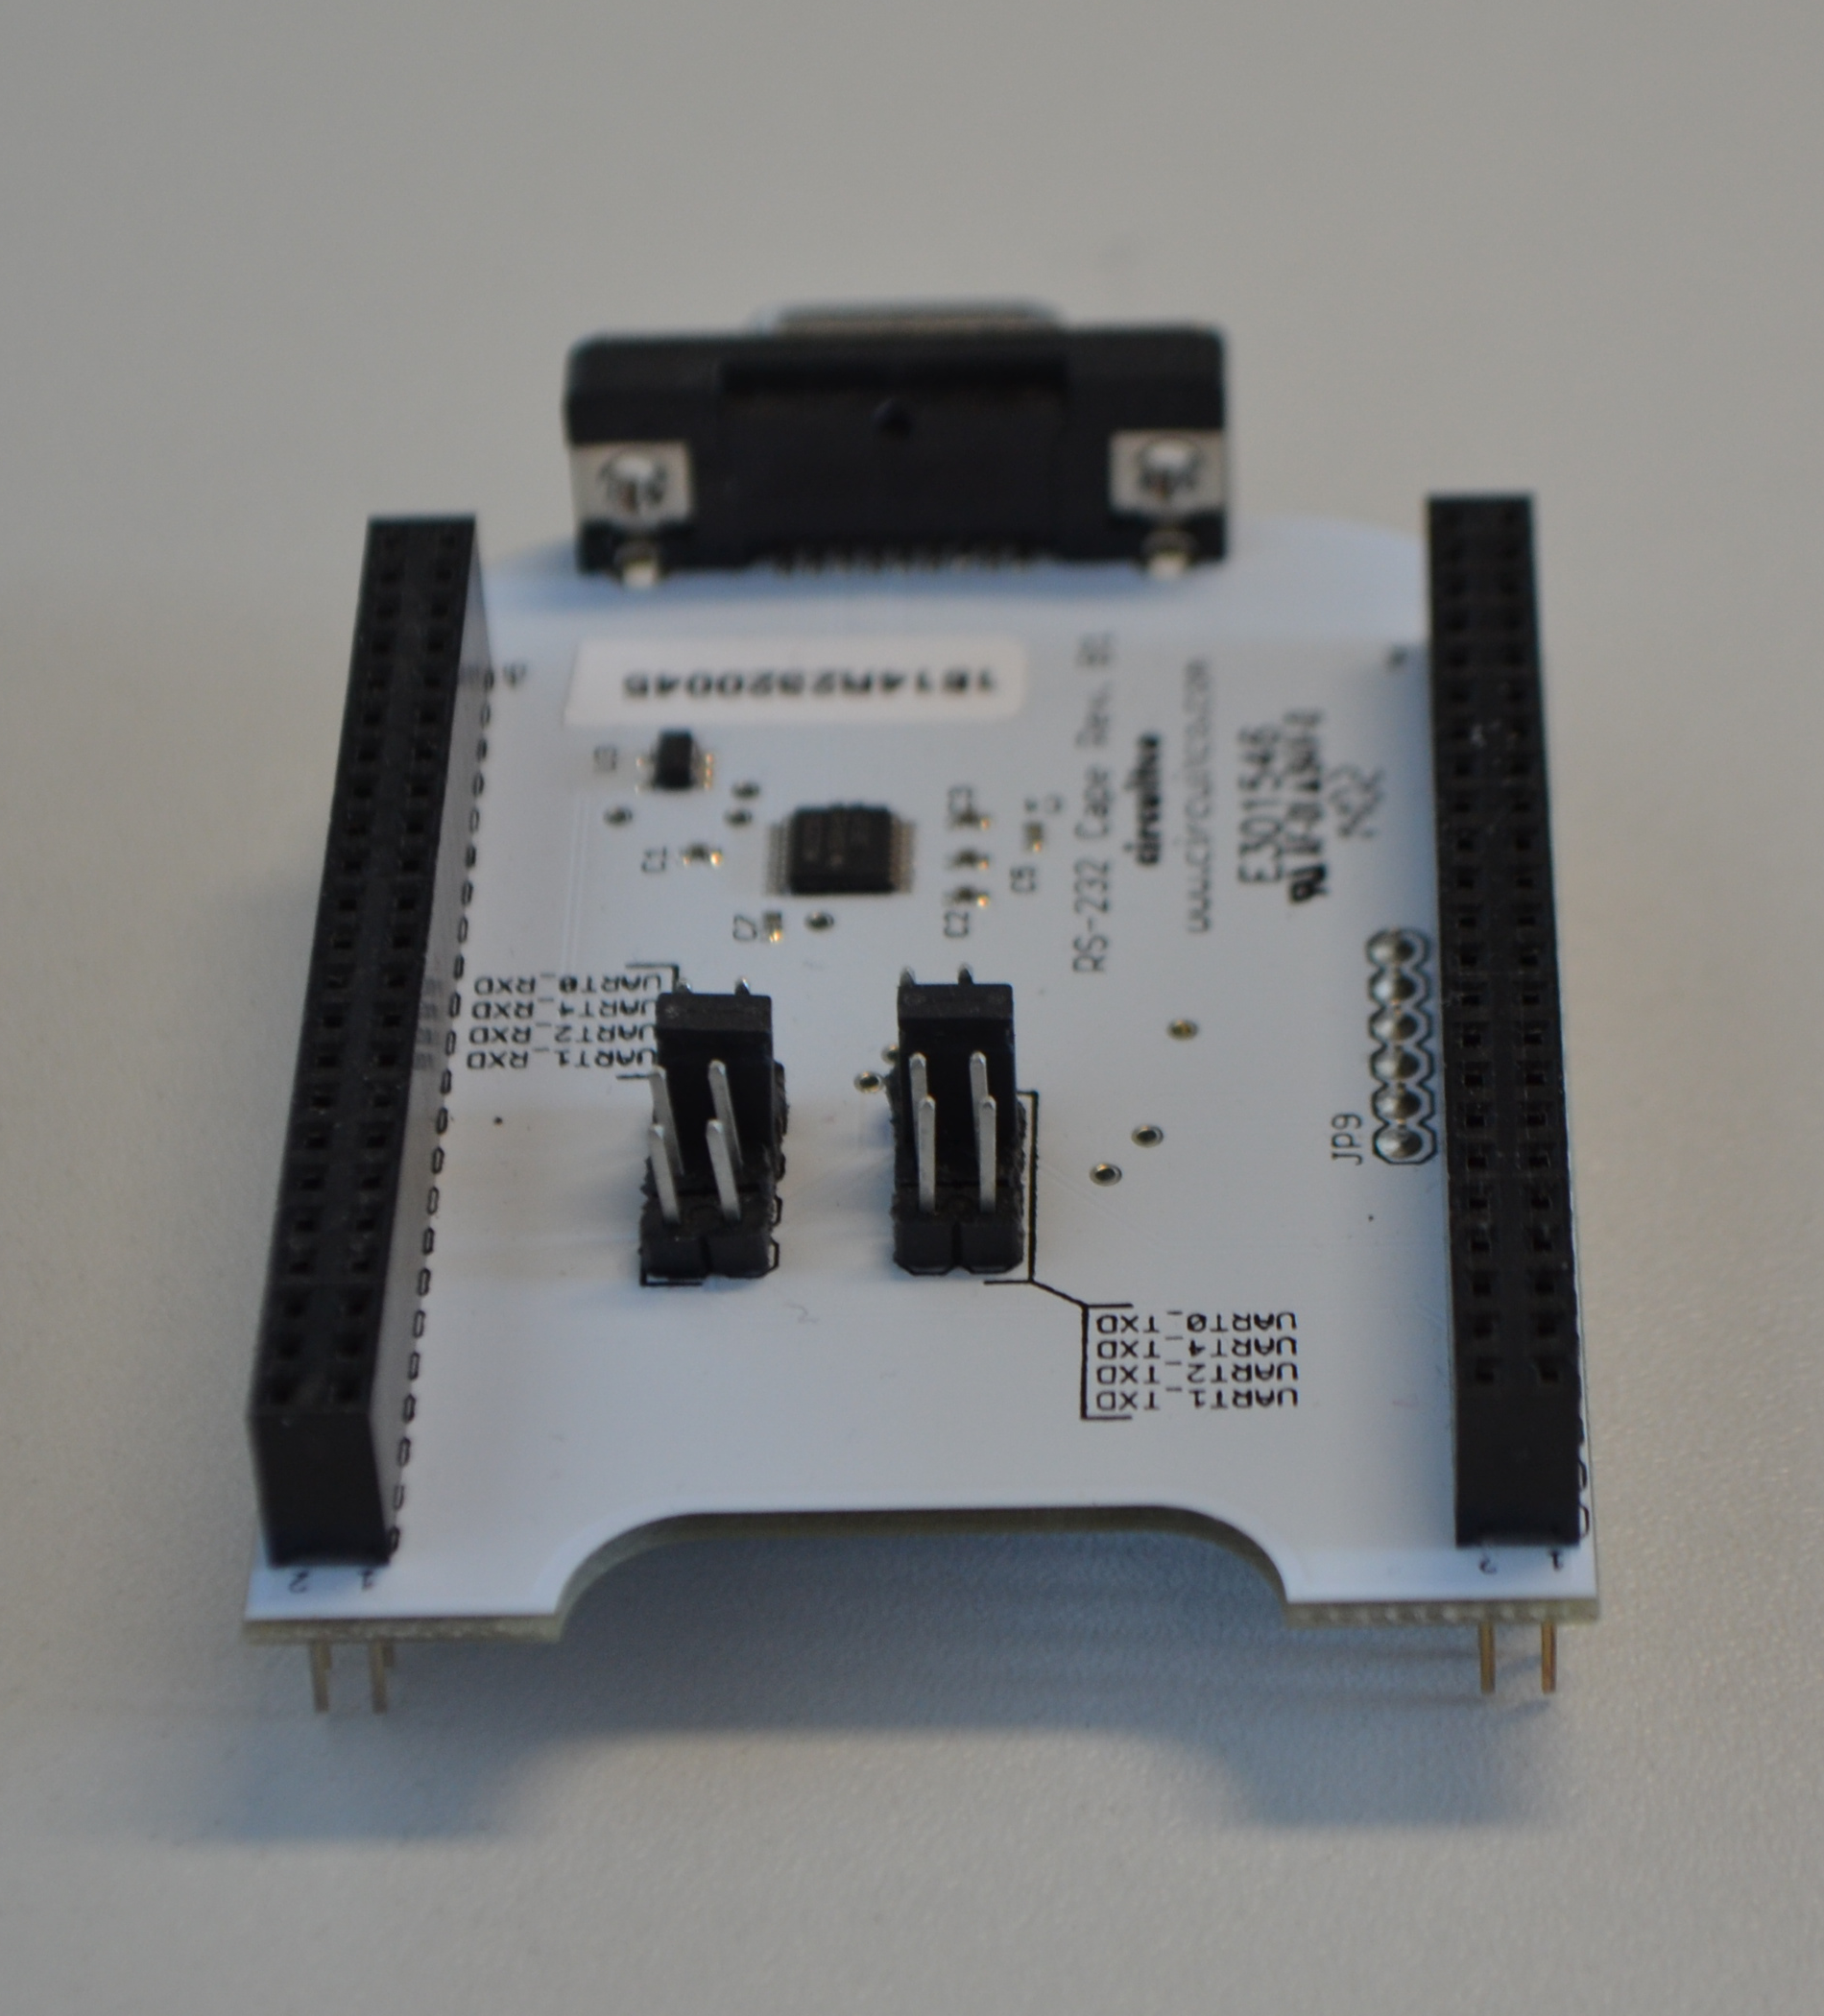
\includegraphics[width=\linewidth]{img/general/CapeRS232.png}
  \caption{RS232 Cape}\label{figure_CapeRS232}
\endminipage\hfill
\minipage{0.32\textwidth}
  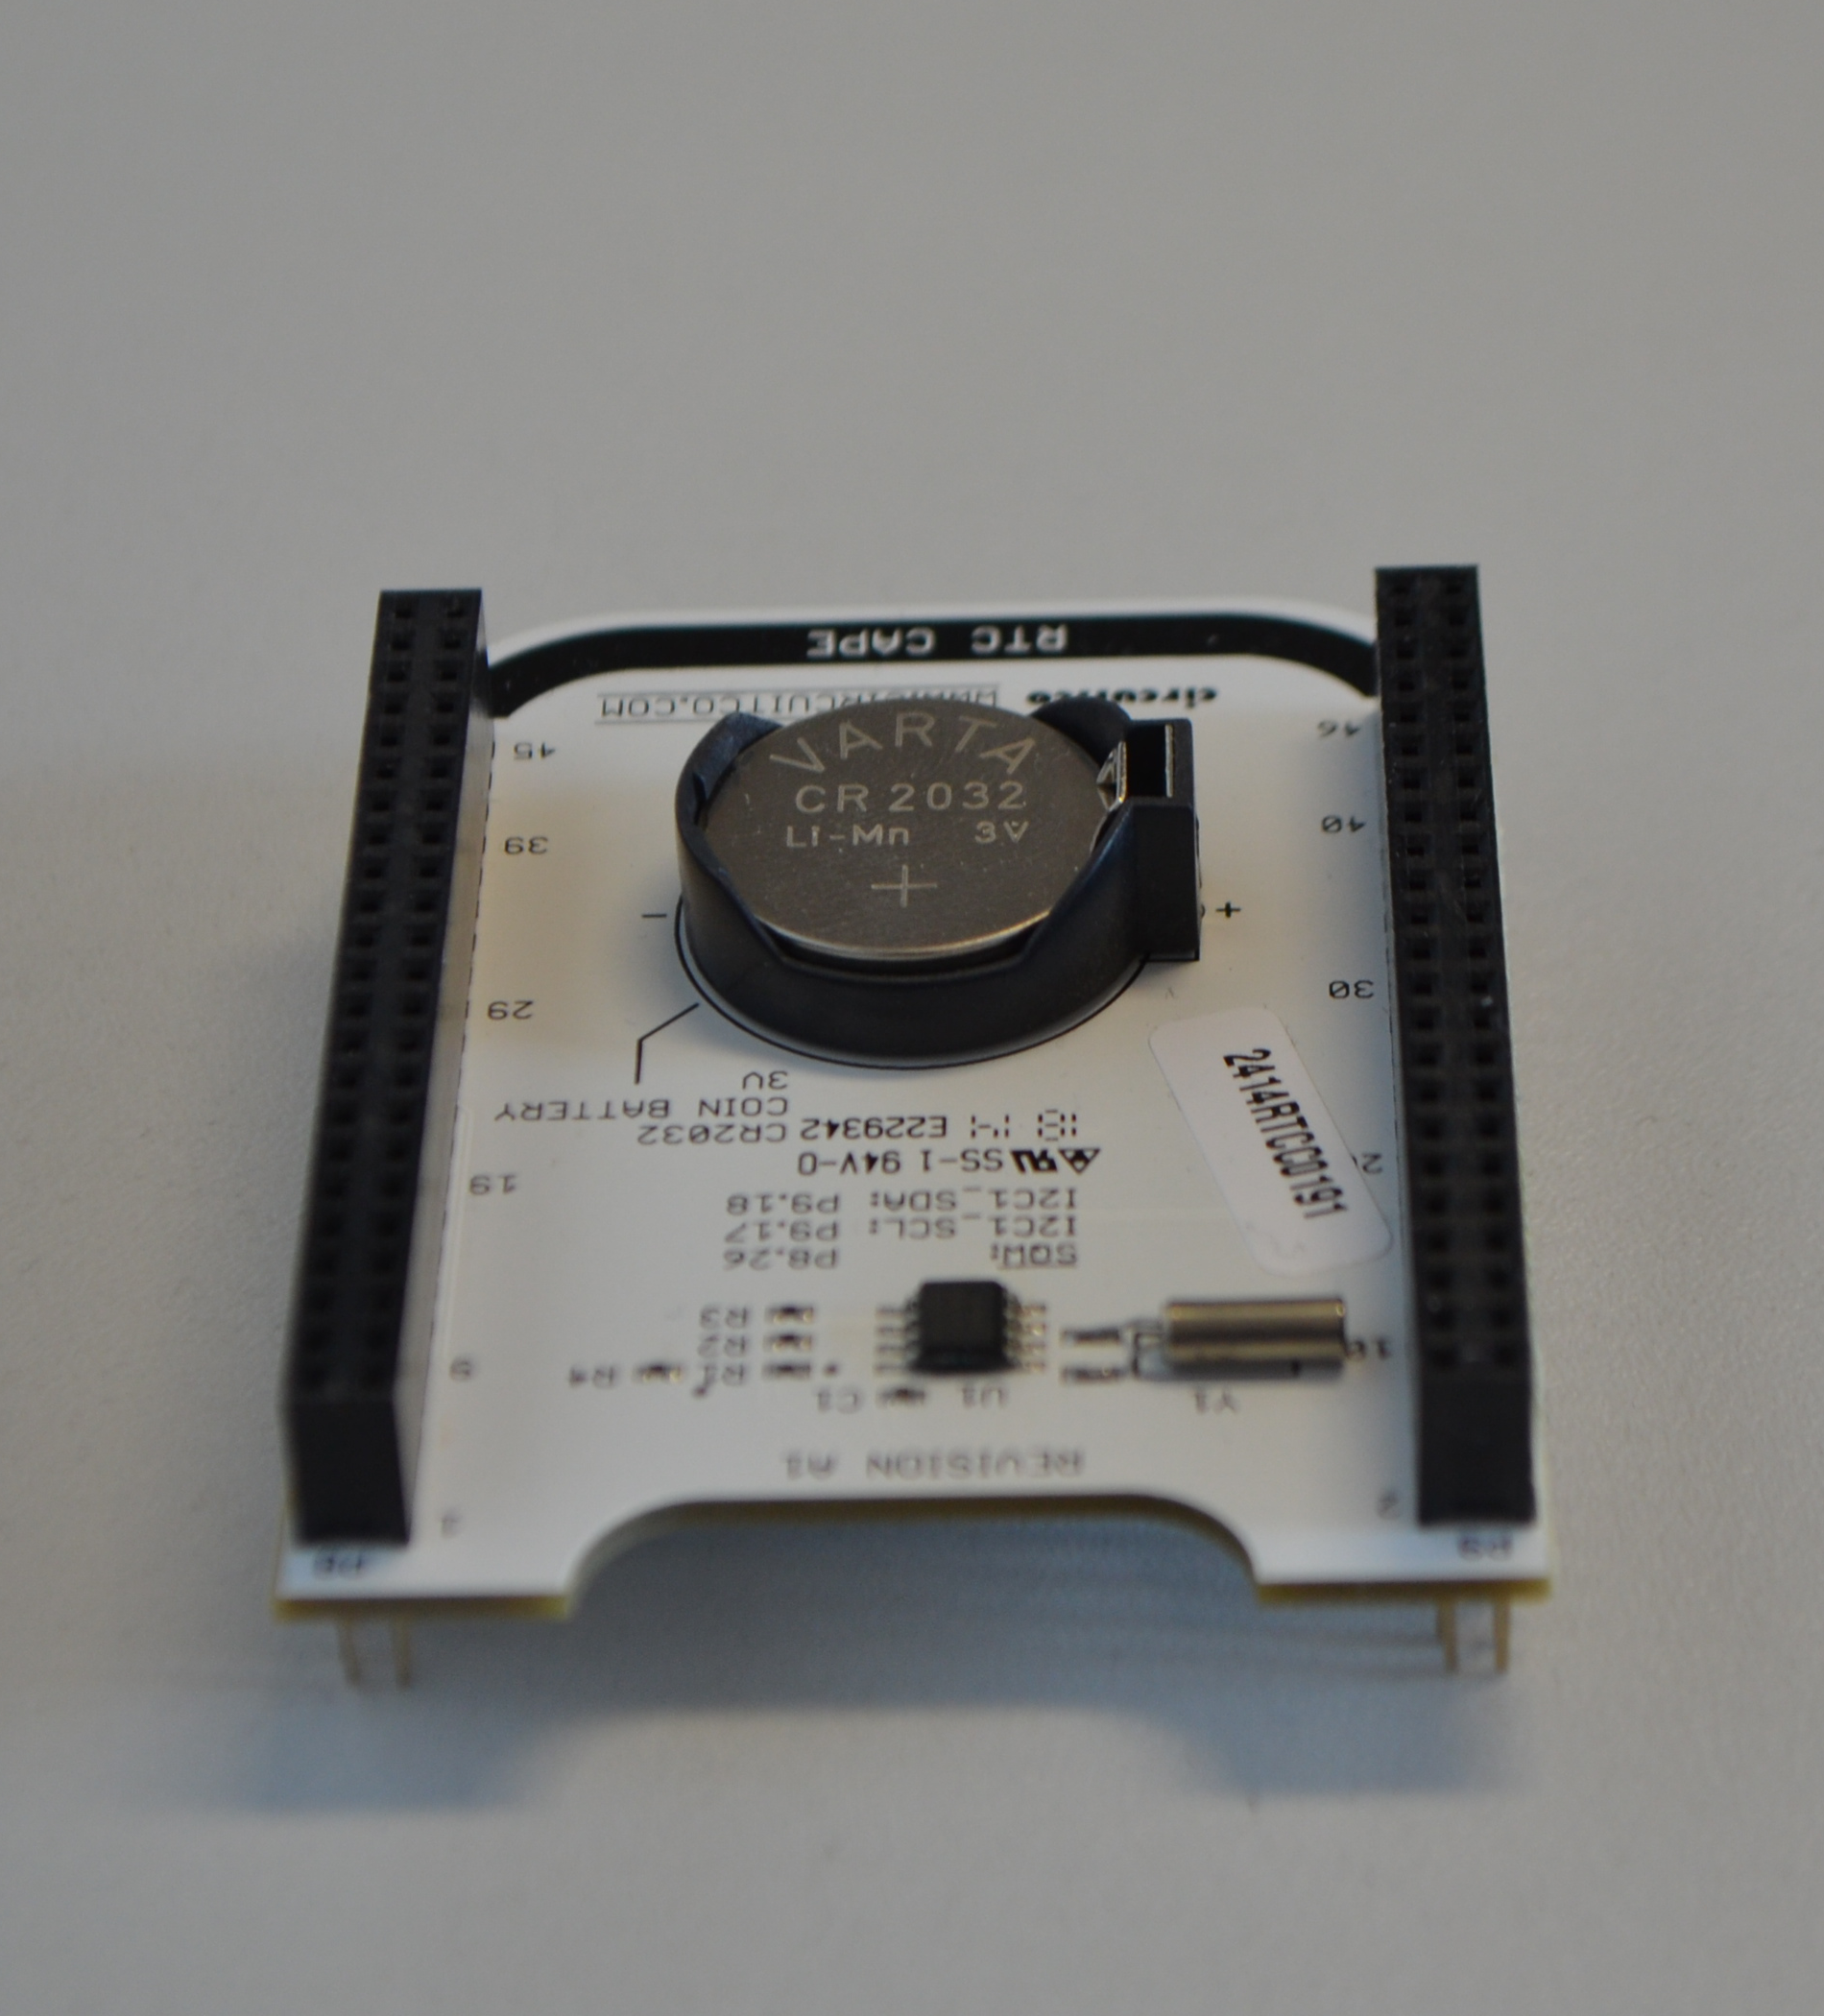
\includegraphics[width=\linewidth]{img/general/CapeRTC.png}
  \caption{RTC Cape}\label{figure_CapeRTC}
\endminipage\hfill
\minipage{0.32\textwidth}%
  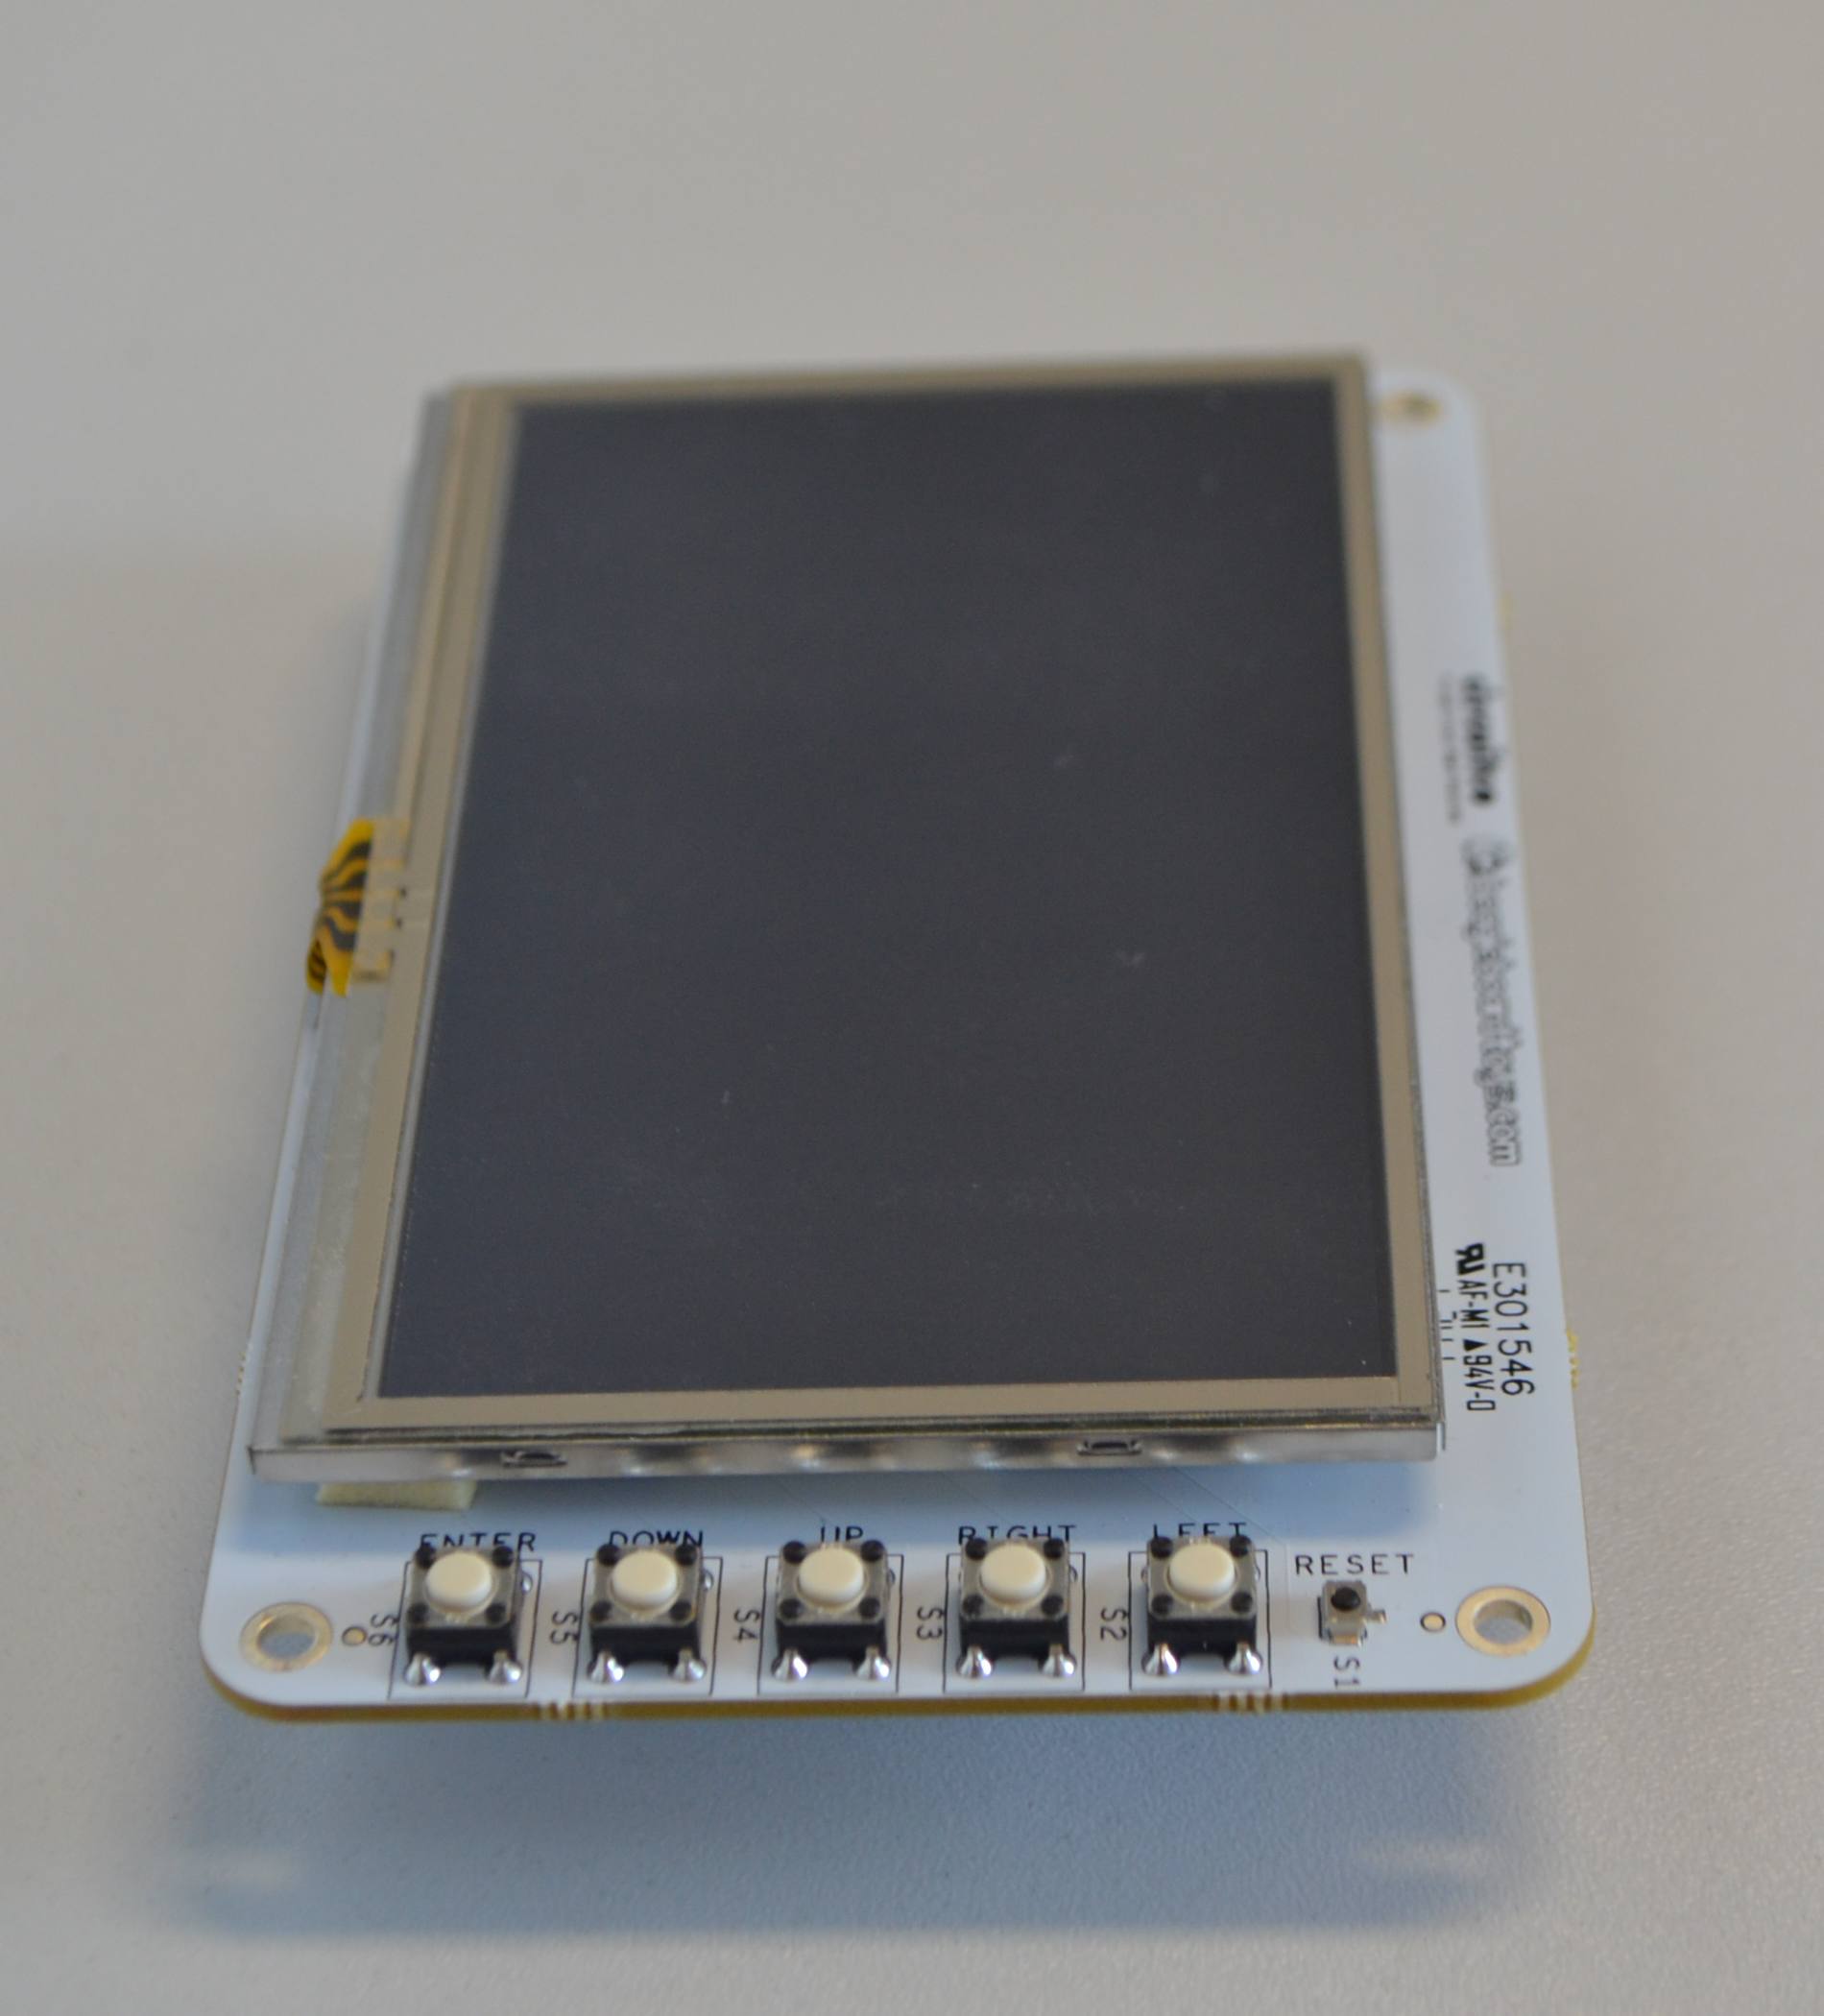
\includegraphics[width=\linewidth]{img/general/CapeLCD.png}
  \caption{LCD Cape}\label{figure_CapeLCD}
\endminipage
\end{figure}


Zur Kommunikation mit den Mess-Clients wird die \ac{UART} Schnittstelle des BeagleBone Black verwendet. Dafür wird ein RS232 Cape eingesetzt (siehe Abbildung \ref{figure_CapeRS232}). Das Cape führt die seriellen Ports UART0, UART1, UART2 und UART4 auf einen 9-poligen seriellen Stecker. Es bietet die Möglichkeit zwischen den verschiedenen Ports mittels eines Jumper auf dem Cape zu wechseln. Angeschlossen wird nach dem 3-wire Prinzip. Dabei werden lediglich Rx, Tx und die Masse verbunden. Somit ist keine Hardware-Flusssteuerung möglich.\ 

Da das BeagleBone Black kein eigenes \ac{RTC} Modul besitzt, wird auch dieses durch ein Cape hinzugefügt (siehe Abbildung \ref{figure_CapeRTC}). Es beinhaltet eine 3V Knopfbatterie um auch im Falle einer Stromunterbrechung die aktuelle Zeit nicht zu verlieren. Dies ist sehr wichtig, da es erforderlich ist, dass das BeagleBone die aktuelle Uhrzeit und das aktuelle Datum jederzeit kennt. Denn beim Erfassen der Messdaten wird ein Zeitstempel angelegt um die Daten später zeitlich zuordnen zu können. Sollte dieser Zeitstempel nicht korrekt sein, sind die Daten bei der Auswertung nicht gültig.\ 

Um die Statusanzeige detailliert darstellen zu können, wird ein resistives LCD-Touchscreen Display eingesetzt. Es hat eine Größe von 4,3 Zoll bei einer Auflösung von 480x272 Pixeln. Dabei handelt es sich ebenso um ein Cape (siehe Abbildung \ref{figure_CapeLCD}) . Dadurch ist es möglich, das BeagleBone Black trotz den Erweiterungen kompakt zu halten. Denn die Capes sind untereinander stapelbar (siehe Abbildung \ref{figure_GestapelteCapes}).\ 


\begin{figure}[H]
\begin{center}
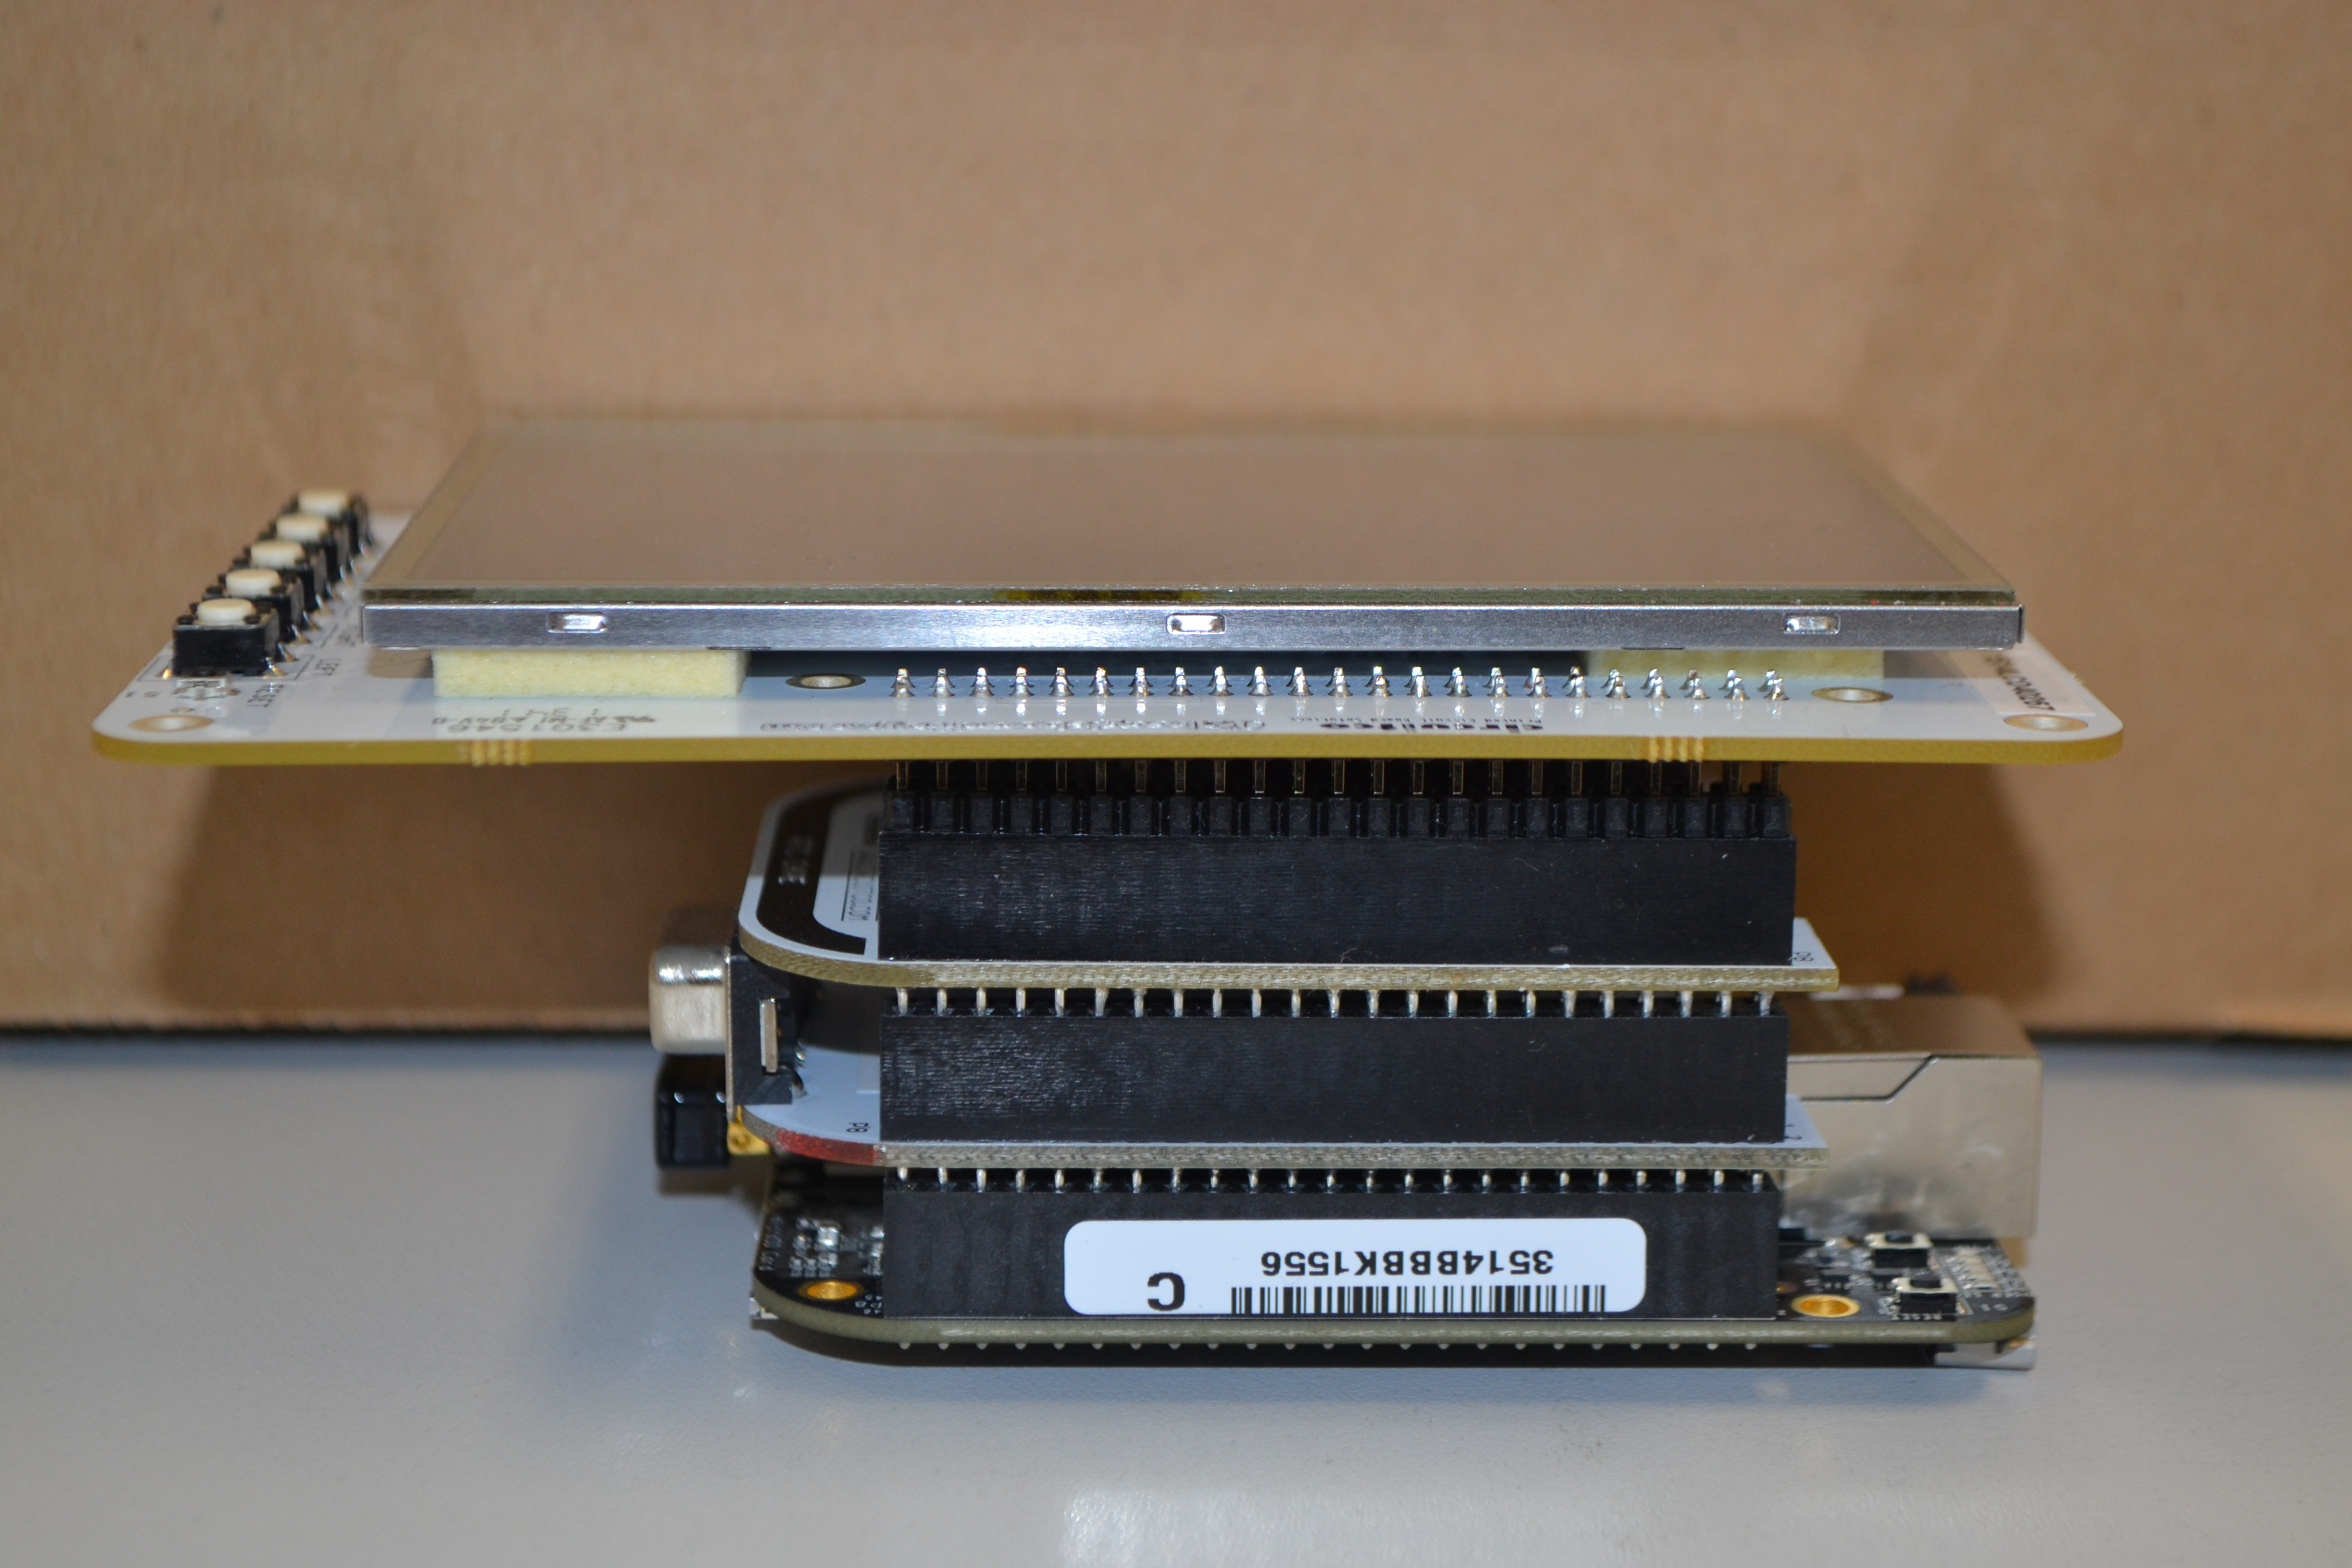
\includegraphics[width=0.5\textwidth ]{img/general/GestapelteCapes.JPG}
\caption{Gestapelte Capes}
\label{figure_GestapelteCapes}
\end{center}
\end{figure}

Die USB Schnittstelle, welche zur Programmierung des BeagleBones verwendet wird, ist bereits vollständig einsatzbereit. Ebenso ist die Ethernet Schnittstelle, welche für den Fernzugriff auf das BeagleBone genutzt wird standardmäßig vollständig integriert.

\section{Software}
\label{ServerSoftware}
Die Programmierung der Software erfolgt in C++ unter Verwendung der Klassenbibliothek Qt (siehe Abschnitt \ref{section_Qt}).\\
Das Softwaredesign teilt sich in einen sequentiellen Teil für die Abfrage und Speicherung der Messwerte, sowie einen Event gesteuerten Teil für die \ac{GUI} und die externe Kommunikation für die Fernzugriffe. Die beiden Programmteile können unabhängig von einander agieren und kommunizieren ausschließlich über Signale und Slots (siehe \ref{QtSignaleSlots}). Durch diese Kapselung ist es möglich die beiden Programmteile durch andere Lösungen auszutauschen, welche lediglich die selben Signale und Slots unterstützen müssen.\ 

\subsection{Messdatenerfassung}
Der Hauptzyklus der Software ruft kontinuierlich die Messdaten von den Mess-Clients ab. Dafür wird ständig geprüft ob Messungen erforderlich sind. Dies geschieht durch den Vergleich der vergangenen Zeit zur letzten Messung und den gegebenen Parametern für die Messintervalle. In der Tabelle \ref{table_ParameterMessintervalle} finden sich diese Parameter.\\


\begin{table}[H]
\begin{center}
\begin{tabular}{|l|l|}\hline
Parameter & Beschreibung \\ \hline
duration\_int1 & Dauer des 1. Zeitraums\\  \hline
duration\_int2 & Dauer des 2. Zeitraums\\  \hline
interval\_1 & Abstand zwischen den Messungen im 1. Zeitraum\\  \hline
interval\_2 & Abstand zwischen den Messungen im 2. Zeitraum\\  \hline
interval\_3 & Abstand zwischen den Messungen nach dem 2. Zeitraum\\ \hline
\end{tabular}
\caption{Parameter der Messintervalle}
\label{table_ParameterMessintervalle}
\end{center}
\end{table}


Ob eine Messung erforderlich ist, lässt sich aus den gegebenen Parametern ableiten. So wird zuerst geprüft, welcher Zeitraum (\textit{duration\_int1-2}) derzeit zutrifft. Dazu wird die vergangene Zeit seit der ersten Messung mit dem Zeitraum abgeglichen. Sollten noch keine Ergebnisse vorhanden sein, ergibt dies die Erforderlichkeit einer Messung. Wenn der passende Zeitraum ausgemacht ist, wird das dazugehörige Intervall zwischen den einzelnen Messungen (\textit{interval\_1-3}) ausgemacht. Dann wird geprüft, ob die vergangene Zeit seit der letzten Messung größer ist als dieses Intervall.\ 

Anschließend wird geprüft ob der Mess-Client verfügbar ist. Dazu wird eine Namensanfrage über die RS232 Schnittstelle verschickt. Bei einer positiven Antwort wird dann eine Messung durchgeführt. Dabei werden alle \acp{ADC} der 64 möglichen \acp{DUT} mittels \textit{ADC-Value}-Befehls (siehe Tabelle \ref{table_Commands}) ausgelesen. Sobald alle 64 Werte erfolgreich ermittelt sind, werden sie in der Datenbank abgelegt. \\
Sollte keine Antwort auf die Namensanfrage erfolgen, wird in den nächsten Zyklen erneut versucht eine Verbindung zu etablieren. Bei kontinuierlich erfolglosen Verbindungsversuchen, informiert das System den Nutzer nach einer festgelegten Zeit der Abwesenheit über die Unerreichbarkeit.
 
\begin{figure}[H]
\begin{center}
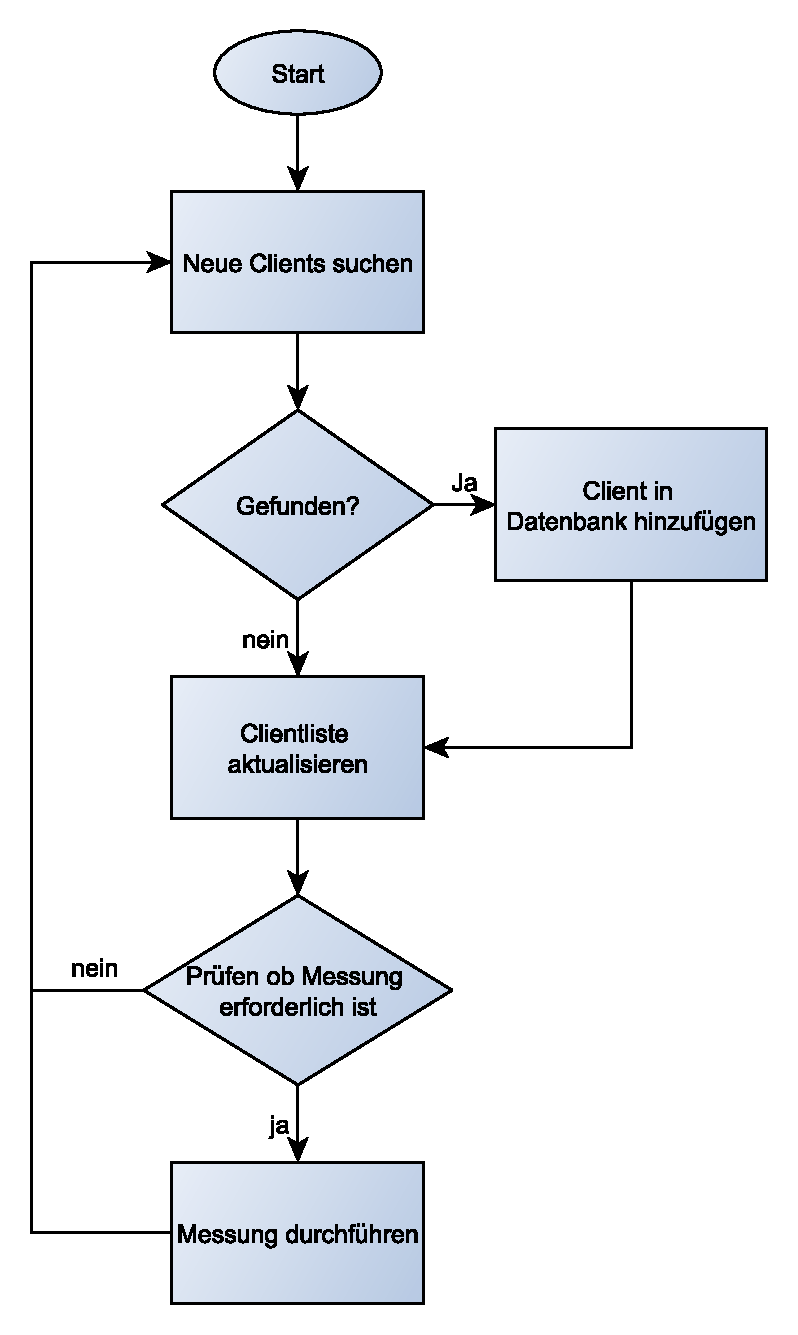
\includegraphics[width=0.5\textwidth ]{img/general/Ablaufplan_Master.pdf}
\caption{Ablaufplan}
\label{figure_Ablaufplan_Master}
\end{center}
\end{figure}
 
\newpage
\subsection{Benutzeroberfläche}
Um die Anforderung der Statusüberwachnung zu erfüllen, verfügt das BeagleBone über eine \ac{GUI}. Sie bietet einen einfachen Überblick über die aktuellen Vorgänge und soll auf einen Blick den Status des Mess-Servers wiedergeben.\\
Am oberen Rand der \ac{GUI} (sieht u.a. Abbildung \ref{figure_MessServerGUIStatus}) wird das aktuelle Datum und die aktuelle Uhrzeit angezeigt, sowie die derzeitige IP Adresse und der aktuelle Name. Am unteren Rand wird die derzeit ausführende Aktion in einer Statusnachricht ausgegeben.
Die \ac{GUI} ist dabei in vier Tabs unterteilt.

\textbf{Status Tab}

\begin{figure}[H]
\begin{center}
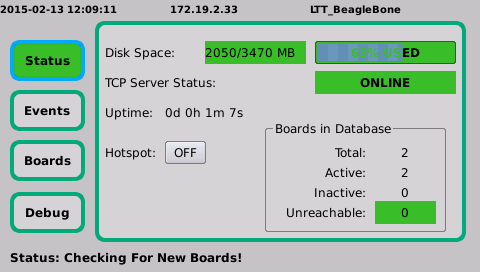
\includegraphics[width=0.5\textwidth ]{img/GUI/Server_GUI_Status1.png}
\caption{Mess-Server GUI: Status Tab}
\label{figure_MessServerGUIStatus}
\end{center}
\end{figure}

Das Erste ist das Status-Tab (siehe Abbildung \ref{figure_MessServerGUIStatus}). Es zeigt die wichtigsten Statusdaten wie verfügbarer Speicher, die aktuelle Laufzeit und TCP Server Status an. Um auf einen Blick den Status des Systems zu erkennen wird mittels der Farben grün und rot ein positiver bzw. negativer Status signalisiert.

\textbf{Events Tab}

\begin{figure}[H]
\begin{center}
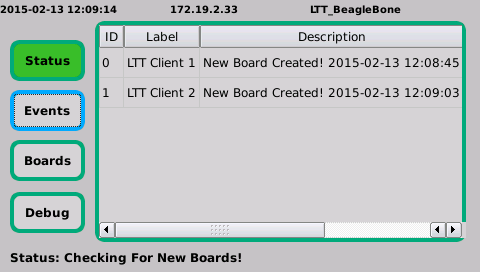
\includegraphics[width=0.5\textwidth ]{img/GUI/Server_GUI_Events1.png}
\caption{Mess-Server GUI: Events Tab}
\label{figure_MessServerGUIEvents}
\end{center}
\end{figure}

Im Events Tab werden wichtige Ereignisse dargestellt. 

\textbf{Boards Tab}

\begin{figure}[H]
\begin{center}
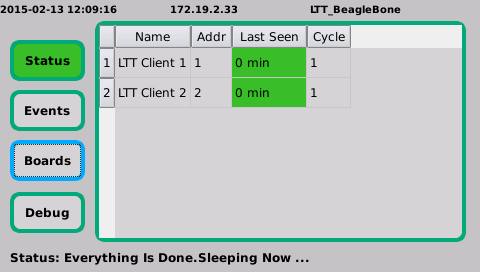
\includegraphics[width=0.5\textwidth ]{img/GUI/Server_GUI_Boards1.png}
\caption{Mess-Server GUI: Boards Tab}
\label{figure_MessServerGUIBoards}
\end{center}
\end{figure}

Das Boards Tab zeigt die derzeit aktiven Mess-Clients in einer Liste an. Als aktiv werden Mess-Clients bezeichnet, die mit einer gültigen Adresse in der Datenbank eingetragen sind. Angezeigt werden der Name, die Adresse, die vergangene Zeit seit dem es das letzten mal erfolgreich kontaktiert wurde und die Anzahl der erfolgreichen aufgenommenen Messzyklen.

\textbf{Debug Tab}

\begin{figure}[H]
\begin{center}
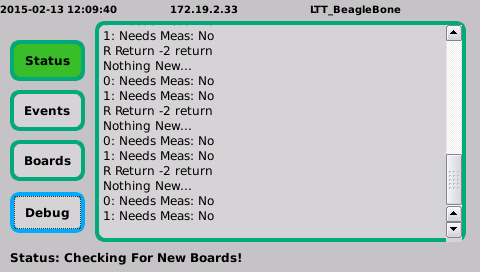
\includegraphics[width=0.5\textwidth ]{img/GUI/Server_GUI_Debug2.png}
\caption{Mess-Server GUI: Debug Tab}
\label{figure_MessServerGUIDebug}
\end{center}
\end{figure}

Der Zweck des Debug Tabs ist es die im Programmcode erzeugten Nachrichten anzuzeigen. Somit soll es möglich sein Fehler einfacher zu erkennen.

\subsection{RS232 Kommunikation}
\label{section_RS232Kommunikation}
Die RS232 Schnittstelle wird ausschließlich zur Kommunikation mit den Mess-Clients verwendet. Um die Erfolgschancen der Anfragen zu erhöhen, werden Fehlschläge erkannt und durch den Versuch des erneuten Sendens minimiert. Zwischen jedem Sendeversuch befindet sich eine kurze Verzögerung.
 
 client anmeldung
 
 client abfrage der werte
 
 

\subsubsection{Ethernet Kommunikation}

Um auf Netzwerkanfragen reagieren zu können, ist sowohl ein UDP-Server für Broadcast-Nachrichten als auch ein TCP-Server für die direkte Kommunikation realisiert.\\
Der UDP-Server dient dabei zur dynamischen Erkennung im Netzwerk. Dabei antwortet der Mess-Server auf Broadcast-Nachrichten mit seiner IP-Adresse und seinem Namen. Dies ermöglicht die einfache Eingliederung der Mess-Server in ein Netzwerk.
Der TCP-Server nimmt RS232- und SQL-Befehle an und leitet diese weiter. Dies ermöglicht den Fernzugriff auf die einzelnen Mess-Clients über ein Netzwerk. 

\begin{table}[H]
\begin{center}
\begin{tabularx}{\textwidth}{|c|c|c|X|}\hline 
 Command & Typ & Daten & Kommentar \\ \hline
 BeagleSendYourIP & UDP & - & Das BeagleBone antwortet dem Sender mit seiner IP Adresse und seinem Namen  \\ \hline
 BeagleUpdateConfig & UDP & - & Das BeagleBone aktualisiert seine Konfiguration aus der Config-Datei \\ \hline
 RS232CMD: & TCP & RS232 Rahmen & Das BeagleBone sende den empfangenen Rahmen über seine RS232 Schnittstelle \\ \hline
 SQLCMD: & TCP & SQL Anfrage & Das BeagleBone führt die SQL Anfrage aus \\ \hline
\end{tabularx}
\caption{Ethernet Befehlsliste}
\label{table_EthernetCommands}
\end{center}
\end{table}

\subsection{Webzugriff}

Um eine Übersicht über die gesammelten Daten auf einem Mess-Server zu erhalten, ist ein lighttpd Webserver installiert.

\subsection{Datenbank}
\label{section_EntwurfDatenbank}

Auf dem  BeagleBone kommt ein MySQL Datenbankserver zum Einsatz. 

Aus den Anforderungen ergibt sich folgendes \ac{ERM} (siehe Abbildung \ref{ERM}). \\

\begin{figure}[H]
\begin{center}
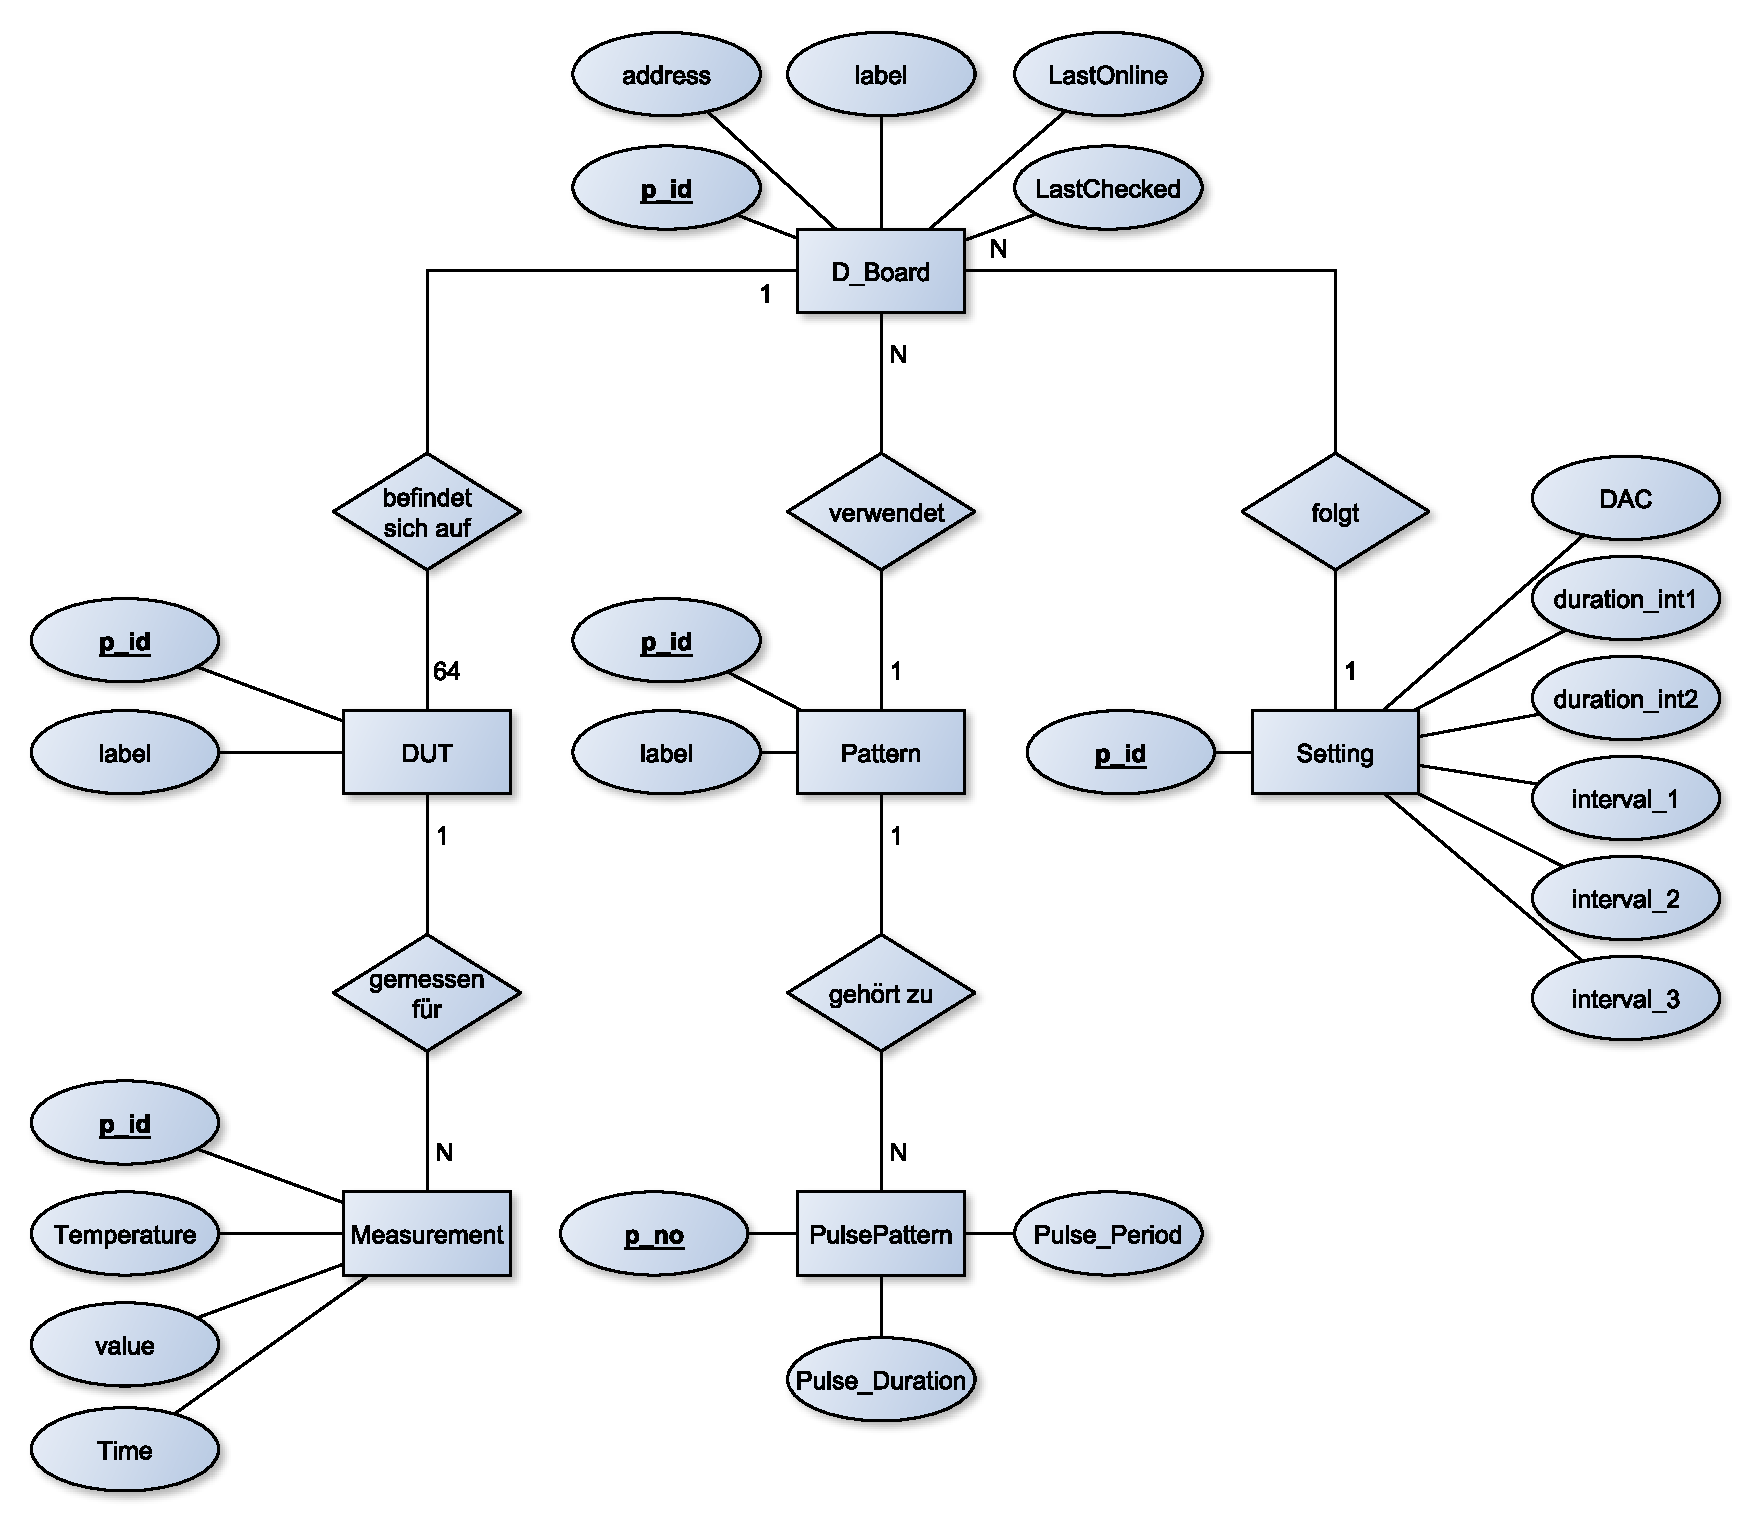
\includegraphics[width=\textwidth]{img/general/ER_Diagramm.pdf}
\caption{Entity Relationship Modell}
\label{ERM}
\end{center}
\end{figure}


Die Datenbank muss folgende Daten für die Parameter der Mess-Clients aufnehmen:\\

\begin{table}[H]
\begin{center}
\begin{tabular}{|l|l|}\hline
Parameter & Beschreibung \\ \hline
DAC & Vorverstärkung\\ 
duration\_int1 & Dauer der Zeit die Werte im 1.Interval aufgenommen werden in Tagen\\ 
duration\_int2 & Dauer der Zeit die Werte im 2.Interval aufgenommen werden in Tagen\\ 
interval\_1 & Abstand zwischen den Messungen im 1. Interval in Minuten\\ 
interval\_2 & Abstand zwischen den Messungen im 2. Interval in Minuten\\ 
interval\_3 & Abstand zwischen den Messungen nach dem 2. Interval in Minuten\\ \hline
\end{tabular}
\caption{Tabelle Setting}
\label{table_TabelleSetting}
\end{center}
\end{table}


